\subsubsection{Core}

\begin{center}
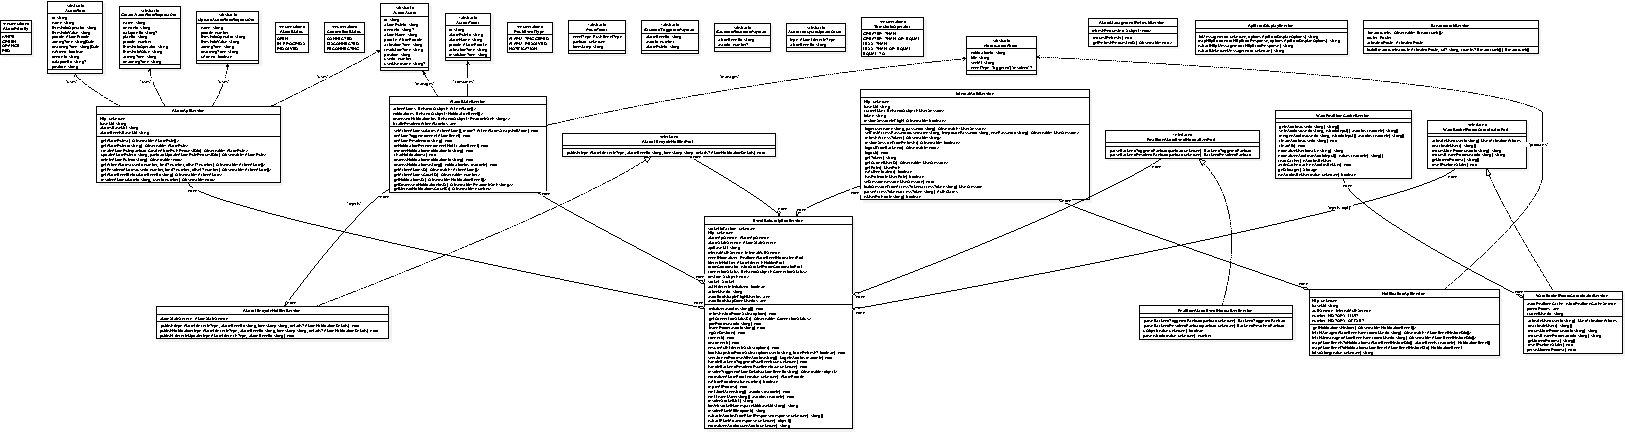
\includegraphics[width=\textwidth]{./frontend/core/core.pdf}
\captionof{figure}{\href{https://snakebyteteam.github.io/3-PB/Documenti_esterni/Specifica_tecnica/frontend/core/core.pdf}{Diagramma delle classi del modulo Core}}
\end{center}

\addAtr{+}{name: string}{}
\addAtr{+}{deviceId: string}{}
\addAtr{+}{datapointId?: string}{}
\addAtr{+}{plantId: string}{}
\addAtr{+}{priority: number}{}
\addAtr{+}{thresholdOperator: string}{}
\addAtr{+}{thresholdValue: string}{}
\addAtr{+}{armingTime: string}{}
\addAtr{+}{dearmingTime: string}{}
\makeAbCl{CreateAlarmRuleRequestDto}{Interfaccia che rappresenta il DTO per la creazione di una nuova regola di allarme. Raccoglie tutti i campi necessari alla definizione della regola, inclusi dispositivo, soglia e orari di armamento.}

\addAtr{+}{name: string}{}
\addAtr{+}{priority: number}{}
\addAtr{+}{thresholdOperator: string}{}
\addAtr{+}{thresholdValue: string}{}
\addAtr{+}{armingTime: string}{}
\addAtr{+}{dearmingTime: string}{}
\addAtr{+}{isArmed: boolean}{}
\makeAbCl{UpdateAlarmRuleRequestDto}{DTO che definisce la struttura dei dati necessaria per aggiornare i parametri di una regola di allarme esistente. Permette di modificare i criteri di soglia, le tempistiche di attivazione e lo stato di armamento del sistema.}

\addAtr{+}{id: string}{}
\addAtr{+}{alarmRuleId: string}{}
\addAtr{+}{deviceId?: string}{}
\addAtr{+}{alarmName: string}{}
\addAtr{+}{priority: AlarmPriority}{}
\addAtr{+}{activationTime: string}{}
\addAtr{+}{resolutionTime: string $|$ null}{}
\addAtr{+}{position: string}{}
\addAtr{+}{userId: number $|$ null}{}
\addAtr{+}{userUsername?: string $|$ null}{}
\makeAbCl{ActiveAlarm}{Questa interfaccia definisce la struttura di un allarme attivo all'interno del sistema, raggruppando informazioni identificative, temporali e di localizzazione. Viene utilizzata per tracciare lo stato degli allarmi in corso, includendo i dettagli sulla priorità e l'eventuale utente assegnato alla risoluzione.}

\addAtr{+}{id: string}{}
\addAtr{+}{alarmRuleId: string}{}
\addAtr{+}{alarmName: string}{}
\addAtr{+}{priority: AlarmPriority}{}
\addAtr{+}{activationTime: string}{}
\addAtr{+}{resolutionTime: string $|$ null}{}
\makeAbCl{AlarmEvent}{Questa interfaccia rappresenta un evento di allarme specifico, contenendo i dati essenziali relativi alla sua attivazione, risoluzione e livello di criticità. Fornisce una struttura standardizzata per tracciare lo storico e lo stato temporale delle notifiche generate dal sistema di monitoraggio.}

\addAtr{+}{id: string}{}
\addAtr{+}{name: string}{}
\addAtr{+}{thresholdOperator: string}{}
\addAtr{+}{thresholdValue: string}{}
\addAtr{+}{priority: AlarmPriority}{}
\addAtr{+}{armingTime: Date $|$ string}{}
\addAtr{+}{dearmingTime: Date $|$ string}{}
\addAtr{+}{isArmed: boolean}{}
\addAtr{+}{deviceId: string}{}
\addAtr{+}{datapointId?: string}{}
\addAtr{+}{position: string}{}
\makeAbCl{AlarmRule}{Questa interfaccia definisce i criteri e le configurazioni di una regola di allarme applicata a un dispositivo o datapoint specifico. Include i parametri operativi come le soglie di intervento, i tempi di attivazione e il livello di priorità per il monitoraggio dei sistemi.}

\addAtr{-}{http: HttpClient}{}
\addAtr{-}{baseUrl: API\_BASE\_URL}{}
\addAtr{-}{alarmsBaseUrl: string}{}
\addAtr{-}{alarmEventsBaseUrl: string}{}
\addMet{+}{getAlarmRules() : Observable$<$AlarmRule[]$>$}{Recupera l'elenco completo di tutte le regole di allarme configurate nel sistema.}
\addMet{+}{getAlarmRule(id: string) : Observable$<$AlarmRule$>$}{Ottiene i dettagli specifici di una singola regola di allarme tramite il suo identificativo univoco.}
\addMet{+}{createAlarmRule(payload: CreateAlarmRuleRequestDto) : Observable$<$AlarmRule$>$}{Crea una nuova regola di allarme inviando i dati di configurazione al server.}
\addMet{+}{updateAlarmRule(id: string, payload: UpdateAlarmRuleRequestDto) : \\ Observable$<$AlarmRule$>$}{Aggiorna i parametri di una regola di allarme esistente identificata dall'ID fornito.}
\addMet{+}{deleteAlarmRule(id: string) : Observable$<$void$>$}{Rimuove definitivamente una regola di allarme dal sistema.}
\addMet{+}{getActiveAlarms(userId: number, limit, offset) : Observable$<$ActiveAlarm[]$>$}{Recupera la lista degli allarmi attivi e non ancora gestiti per un determinato utente con supporto alla paginazione.}
\addMet{+}{getResolvedAlarms(userId: number, limit, offset) : Observable$<$ActiveAlarm[]$>$}{Ritorna lo storico degli allarmi già risolti e gestiti da uno specifico utente.}
\addMet{+}{getAlarmEventById(alarmEventId: string) : Observable$<$ActiveAlarm$>$}{Recupera le informazioni dettagliate di uno specifico evento di allarme tramite il suo ID.}
\addMet{+}{resolveAlarm(alarmId: string, userId: number) : Observable$<$void$>$}{Invia la richiesta per marcare un allarme specifico come risolto dall'utente indicato.}
\makeCl{AlarmApiService}{Questa classe di servizio gestisce tutte le comunicazioni HTTP relative alle regole di allarme e agli eventi di allarme verso l'API di backend. Centralizza le operazioni di CRUD per le configurazioni e il monitoraggio degli stati di attivazione e risoluzione degli allarmi.}

\addAtr{+}{alarmName?: string}{}
\addAtr{+}{priority?: unknown}{}
\makeAbCl{AlarmNotificationDetails}{Questa interfaccia definisce i dettagli opzionali necessari per la costruzione del contenuto informativo di una notifica di allarme. Permette di trasportare il nome della regola e il suo livello di priorità per una visualizzazione corretta all'utente.}


\addMet{+}{publish(type: AlarmLifecycleType, alarmEventId: string, \\ timestamp: string, details?: AlarmNotificationDetails): void}{Definisce il contratto per la pubblicazione degli eventi legati al ciclo di vita di un allarme verso i sistemi di notifica.}
\makeItf{AlarmLifecycleNotifierPort}{Interfaccia di porta che astrae il meccanismo di notifica del ciclo di vita degli allarmi, permettendo l'invio di aggiornamenti su attivazioni e risoluzioni. Facilita il disaccoppiamento tra la logica di business e l'implementazione specifica della distribuzione degli eventi.}


\addAtr{-}{alarmStateService: AlarmStateService}{}
\addMet{+}{publish(type: AlarmLifecycleType, alarmEventId: string, \\ timestamp: string, details?: AlarmNotificationDetails): void}{Coordina il processo di notifica globale attivando sia la creazione della notifica visiva che l'aggiornamento dello stato del ciclo di vita.}
\addMet{-}{publishNotification(type: AlarmLifecycleType, alarmEventId: string, \\ timestamp: string, details?: AlarmNotificationDetails): void}{Costruisce e invia una notifica formattata al servizio di stato degli allarmi in base al tipo di evento ricevuto.}
\addMet{-}{publishLifecycleUpdate(type: AlarmLifecycleType, alarmEventId: string): void}{Emette un evento personalizzato a livello globale per informare i componenti dell'applicazione dell'avvenuta modifica di un allarme.}
\makeCl{AlarmLifecycleNotifierService}{Questo servizio implementa la logica per la gestione delle notifiche in tempo reale e degli aggiornamenti di stato relativi agli allarmi. Centralizza la creazione dei titoli delle notifiche e l'invio degli eventi tramite il dispatcher globale dell'applicazione.}

\addAtr{-}{refreshRequested\$: Subject$<$void$>$}{}
\addMet{+}{requestRefresh() : void}{Innesca una nuova richiesta di aggiornamento emettendo un segnale attraverso il relativo stream.}
\addMet{+}{getRefreshRequested\$() : Observable$<$void$>$}{Restituisce un Observable che permette ai componenti di sottoscriversi per reagire alle richieste di refresh.}
\makeCl{AlarmManagementRefreshService}{Questo servizio fornisce un meccanismo centralizzato per coordinare l'aggiornamento dei dati relativi alla gestione degli allarmi all'interno dell'applicazione. Permette la comunicazione disaccoppiata tra diversi componenti che necessitano di sincronizzare il rinfresco delle interfacce.}

\addAtr{-}{activeAlarms\$: BehaviorSubject$<$ActiveAlarm[]$>$}{}
\addAtr{-}{notifications\$: BehaviorSubject$<$NotificationEvent[]$>$}{}
\addAtr{-}{dismissedNotificationIds\$: BehaviorSubject$<$ReadonlySet$<$string$>>$}{}
\addAtr{-}{locallyResolvedActiveAlarmIds: Set$<$string$>$}{}
\addMet{+}{setActiveAlarms(alarms: ActiveAlarm[], mode: ActiveAlarmsSnapshotMode): void}{Aggiorna lo stato degli allarmi attivi permettendo di unire i nuovi dati a quelli esistenti o di sostituirli completamente.}
\addMet{+}{onAlarmTriggered(event: AlarmEvent): void}{Gestisce l'attivazione di un nuovo allarme aggiungendolo alla lista locale e resettando eventuali stati di risoluzione precedente.}
\addMet{+}{onAlarmResolved(id: string): void}{Marca un allarme come risolto rimuovendolo dalla lista degli allarmi attivi e tenendo traccia dell'operazione a livello locale.}
\addMet{+}{onNotificationReceived(event: NotificationEvent): void}{Registra la ricezione di una nuova notifica verificando che non sia stata precedentemente scartata dall'utente.}
\addMet{+}{removeNotification(notificationId: string): void}{Elimina una specifica notifica dall'elenco visualizzato e la aggiunge a quelle rimosse definitivamente.}
\addMet{+}{clearNotifications(): void}{Rimuove istantaneamente tutte le notifiche correnti e le marca come scartate nel sistema.}
\addMet{+}{dismissNotification(notificationId: string): void}{Aggiunge l'identificativo di una singola notifica alla lista di quelle ignorate per evitarne la ricomparsa.}
\addMet{+}{dismissNotifications(notificationIds: ReadonlyArray$<$string$>$): void}{Gestisce l'inserimento massivo di più notifiche nella lista di quelle ignorate tramite un'operazione atomica.}
\addMet{+}{getActiveAlarms\$() : Observable$<$ActiveAlarm[]$>$}{Fornisce uno stream osservabile per monitorare in tempo reale i cambiamenti nella lista degli allarmi attivi.}
\addMet{+}{getActiveAlarmsCount\$() : Observable$<$number$>$}{Restituisce un osservabile che emette il numero totale di allarmi attualmente attivi nel sistema.}
\addMet{+}{getNotifications\$() : Observable$<$NotificationEvent[]$>$}{Permette di sottoscriversi per ricevere aggiornamenti sulla lista delle notifiche correnti non ancora rimosse.}
\addMet{+}{getDismissedNotificationIds\$() : Observable$<$ReadonlySet$<$string$>>$}{Restituisce l'insieme degli identificativi delle notifiche che l'utente ha scelto di ignorare.}
\addMet{+}{getUnreadNotificationsCount\$() : Observable$<$number$>$}{Ritorna il conteggio delle notifiche presenti nell'elenco degli avvisi correnti.}
\makeCl{AlarmStateService}{Questo servizio centralizza la gestione dello stato reattivo degli allarmi e delle notifiche all'interno del frontend dell'applicazione. Si occupa di mantenere la sincronia tra gli eventi ricevuti in tempo reale, le azioni dell'utente e la visualizzazione corretta dei contatori e delle liste.}

\addAtr{-}{socketIoFactory: typeof io}{}
\addAtr{-}{http: HttpClient}{}
\addAtr{-}{alarmApiService: AlarmApiService}{}
\addAtr{-}{alarmStateService: AlarmStateService}{}
\addAtr{-}{apiBaseUrl: API\_BASE\_URL}{}
\addAtr{-}{internalAuthService: InternalAuthService}{}
\addAtr{-}{eventNormalizer: RealtimeAlarmEventNormalizerPort}{}
\addAtr{-}{lifecycleNotifier: AlarmLifecycleNotifierPort}{}
\addAtr{-}{roomCoordinator: WardSocketRoomCoordinatorPort}{}
\addAtr{-}{connectionStatus\$: BehaviorSubject$<$ConnectionStatus$>$}{}
\addAtr{-}{destroy\$: Subject$<$void$>$}{}
\addAtr{-}{socket: Socket $|$ null}{}
\addAtr{-}{authLifecycleInitialized: boolean}{}
\addAtr{-}{activeUserId: string $|$ null}{}
\addAtr{-}{wardBootstrapInFlightUserIds: Set$<$string$>$}{}
\addAtr{-}{wardBootstrapDoneUserIds: Set$<$string$>$}{}
\addMet{+}{initialize(wardIds: string[]): void}{Configura la connessione iniziale ai socket, sottoscrive il ciclo di vita dell'autenticazione e unisce l'utente alle stanze dei reparti specificati.}
\addMet{+}{refreshWardRoomSubscription(): void}{Forza l'aggiornamento delle iscrizioni alle stanze dei reparti per l'utente attualmente attivo.}
\addMet{+}{getConnectionStatus\$(): Observable$<$ConnectionStatus$>$}{Restituisce uno stream osservabile per monitorare lo stato della connessione WebSocket in tempo reale.}
\addMet{+}{joinRoom(wardId: string): void}{Richiede l'iscrizione a una specifica stanza di reparto tramite il protocollo socket.}
\addMet{+}{leaveRoom(wardId: string): void}{Invia una richiesta al server per abbandonare la stanza associata a un determinato reparto.}
\addMet{+}{ngOnDestroy(): void}{Gestisce la pulizia delle risorse chiudendo la connessione socket e completando gli stream alla distruzione del servizio.}
\addMet{-}{connect(): void}{Inizializza la connessione WebSocket impostando i gestori degli eventi per la riconnessione e la ricezione dei messaggi dal backend.}
\addMet{-}{disconnect(): void}{Chiude la connessione attiva, rimuove i listener e resetta lo stato interno del coordinatore delle stanze.}
\addMet{-}{ensureAuthLifecycleSubscription(): void}{Sottoscrive i cambiamenti dello stato dell'utente per gestire automaticamente l'ingresso o l'uscita dalle stanze in base alla sessione.}
\addMet{-}{bootstrapWardRoomSubscription(userId: string, forceRefresh: boolean): void}{Esegue il recupero iniziale dei reparti disponibili tramite API per configurare le sottoscrizioni socket dell'utente.}
\addMet{-}{syncJoinedRoomsWithWardIds(targetWardIds: ReadonlyArray$<$string$>$): void}{Sincronizza le stanze attualmente seguite con un nuovo elenco di reparti target, abbandonando quelle non più necessarie.}
\addMet{-}{handleBackendTriggeredRawEvent(raw: unknown): void}{Processa i dati grezzi di un allarme attivato, normalizzandoli e notificando il sistema di stato e il ciclo di vita.}
\addMet{-}{handleBackendResolvedRawEvent(raw: unknown): void}{Gestisce la ricezione di un evento di risoluzione allarme, aggiornando lo stato locale e i notificatori.}
\addMet{-}{resolveTriggeredAlarmDetails(alarmEventId: string): Observable$<$...$>$}{Recupera i dettagli informativi di un allarme dal server per arricchire l'evento ricevuto in tempo reale.}
\addMet{-}{normalizeAlarmPriority(value: unknown): AlarmPriority $|$ null}{Converte e valida i valori di priorità provenienti dal backend nel formato enumerato corretto.}
\addMet{-}{isAlarmPriority(value: number): value is AlarmPriority}{Verifica se un valore numerico corrisponde a uno dei livelli di priorità validi definiti nell'applicazione.}
\addMet{-}{rejoinAllRooms(): void}{Invia nuovamente i comandi di join per tutte le stanze precedentemente attive in seguito a una riconnessione.}
\addMet{-}{emitJoinMany(wardIds: ReadonlyArray$<$string$>$): void}{Invia in blocco comandi di ingresso per una lista di identificativi di reparto.}
\addMet{-}{emitLeaveMany(wardIds: ReadonlyArray$<$string$>$): void}{Invia in blocco comandi di uscita per una lista di identificativi di reparto.}
\addMet{-}{resolveSocketUrl(): string}{Determina l'URL corretto per la connessione WebSocket basandosi sulla configurazione dell'API base.}
\addMet{-}{toWebsocketNamespaceUrl(baseUrl: string): string}{Trasforma un URL API standard nel formato richiesto per il namespace dei WebSocket.}
\addMet{-}{resolvePlantAllEndpoint(): string}{Costruisce l'endpoint URL necessario per recuperare l'elenco di tutti i reparti (plants).}
\addMet{-}{extractWardIdsFromPlantResponse(response: unknown): string[]}{Analizza la risposta del server per estrarre una lista univoca di identificativi di reparto.}
\addMet{-}{extractPlantArray(response: unknown): Array$<$...$>$}{Estrae in modo sicuro l'array di dati dei reparti da diverse possibili strutture di risposta JSON.}
\addMet{-}{normalizeWardId(rawWardId: unknown): string $|$ null}{Normalizza l'identificativo di un reparto convertendolo in una stringa valida o restituendo null.}
\makeCl{EventSubscriptionService}{Questo servizio coordina la comunicazione in tempo reale tramite WebSocket, gestendo le sottoscrizioni alle stanze dei reparti e la ricezione degli eventi di allarme. Si occupa di mantenere la sincronia tra la sessione dell'utente, i dati del database e le notifiche live integrate nel sistema.}

\addMet{+}{parseBackendTriggeredPayload(payload: unknown): BackendTriggeredPayload $|$ null}{Valida e converte i dati grezzi ricevuti dal backend relativi all'attivazione di un nuovo allarme in un oggetto tipizzato.}
\addMet{+}{parseBackendResolvedPayload(payload: unknown): BackendResolvedPayload $|$ null}{Esegue il parsing dei dati grezzi riguardanti la risoluzione di un allarme, assicurando l'integrità dei campi obbligatori.}
\makeItf{RealtimeAlarmEventNormalizerPort}{Interfaccia di porta che definisce il contratto per la normalizzazione dei messaggi ricevuti in tempo reale tramite protocolli di comunicazione asincrona. Garantisce che i dati provenienti dall'esterno siano validati prima di essere processati dalla logica di business.}

\addMet{+}{parseBackendTriggeredPayload(payload: unknown): BackendTriggeredPayload $|$ null}{Implementa la logica di estrazione e validazione per i payload di attivazione allarme, gestendo la conversione degli identificativi di reparto.}
\addMet{+}{parseBackendResolvedPayload(payload: unknown): BackendResolvedPayload $|$ null}{Analizza il contenuto dei messaggi di risoluzione allarme, estraendo l'identificativo dell'evento e il relativo reparto associato.}
\addMet{-}{isObject(value: unknown): value is Record$<$string, unknown$>$}{Verifica internamente se un valore sconosciuto è un oggetto non nullo compatibile con un record di chiavi e valori.}
\addMet{-}{parseWardId(value: unknown): number $|$ null}{Tenta di convertire un valore di input in un identificativo numerico intero valido per la gestione dei reparti.}
\makeCl{RealtimeAlarmEventNormalizerService}{Servizio responsabile della trasformazione e validazione dei dati grezzi in arrivo dal backend via socket in strutture dati coerenti per l'applicazione. Centralizza i controlli di tipo e le conversioni di formato per prevenire errori di runtime dovuti a payload malformati.}

\addMet{+}{getWardIds(userId: string) : string[]}{Recupera dalla cache l'elenco degli identificativi di reparto associati a uno specifico utente.}
\addMet{+}{setWardIds(userId: string, wardIds: ReadonlyArray$<$WardIdInput$>$) : string[]}{Sovrascrive la lista dei reparti per l'utente indicato, normalizzando i valori prima della memorizzazione.}
\addMet{+}{mergeWardIds(userId: string, wardIds: ReadonlyArray$<$WardIdInput$>$) : string[]}{Unisce i nuovi identificativi di reparto a quelli già presenti nella cache per l'utente specificato.}
\addMet{+}{clearWardIds(userId: string) : void}{Rimuove definitivamente dalla cache tutte le informazioni relative ai reparti di un singolo utente.}
\addMet{+}{clearAll() : void}{Svuota completamente lo storage locale rimuovendo ogni dato salvato dal servizio di caching.}
\addMet{-}{normalizeUserId(value: string) : string}{Rimuove gli spazi bianchi in eccesso dall'identificativo utente per garantire la coerenza delle chiavi.}
\addMet{-}{normalizeWardIds(values: ReadonlyArray$<$WardIdInput$>$) : string[]}{Converte i valori di input in una lista di stringhe univoche e validate, eliminando duplicati e valori nulli.}
\addMet{-}{readCache() : WardIdsByUser}{Legge e deserializza i dati dalla session storage, gestendo eventuali errori di parsing o formati non validi.}
\addMet{-}{writeCache(cache: WardIdsByUser) : void}{Serializza e salva lo stato corrente della cache nella session storage del browser.}
\addMet{-}{getStorage() : Storage $|$ null}{Fornisce un riferimento sicuro alla session storage globale dell'ambiente di esecuzione.}
\addMet{-}{isWardIdsByUser(value: unknown) : value is WardIdsByUser}{Esegue una validazione strutturale profonda per assicurarsi che i dati caricati corrispondano al formato atteso dal servizio.}
\makeCl{WardRealtimeCacheService}{Questo servizio gestisce la persistenza temporanea degli identificativi di reparto su base utente utilizzando la session storage del browser. Assicura che le preferenze di monitoraggio in tempo reale siano mantenute durante la sessione, offrendo metodi per la normalizzazione, il recupero e la sincronizzazione dei dati.}

\addAtr{+}{roomsToLeave: string[]}{}
\addAtr{+}{roomsToJoin: string[]}{}
\makeAbCl{UserActivationActions}{Questa interfaccia definisce la struttura degli insiemi di stanze socket da gestire durante la transizione di sessione di un utente. Specifica quali canali devono essere abbandonati e quali attivati per garantire la corretta ricezione degli eventi in tempo reale.}

\addMet{+}{activateUser(userId: string): UserActivationActions}{Gestisce la transizione di un utente calcolando le stanze da abbandonare e quelle da sottoscrivere in base alla cache.}
\addMet{+}{deactivateUser(): string[]}{Esegue il logout dell'utente corrente rimuovendo le informazioni dalla cache e restituendo l'elenco delle stanze da abbandonare.}
\addMet{+}{requestJoinRoom(wardId: string): string $|$ null}{Verifica se l'iscrizione a una nuova stanza di reparto è necessaria e, in caso positivo, la registra nello stato interno.}
\addMet{+}{requestLeaveRoom(wardId: string): string $|$ null}{Rimuove un reparto dallo stato di monitoraggio attivo e restituisce l'identificativo se l'operazione è andata a buon fine.}
\addMet{+}{getJoinedRooms(): string[]}{Restituisce l'elenco completo di tutti gli identificativi di reparto attualmente monitorati dall'istanza attiva.}
\addMet{+}{resetRuntimeState(): void}{Ripristina lo stato iniziale del coordinatore azzerando l'utente corrente e svuotando l'elenco delle stanze attive.}
\makeItf{WardSocketRoomCoordinatorPort}{Interfaccia di porta che definisce la logica di coordinamento per la gestione delle stanze socket associate ai reparti ospedalieri. Astrae la complessità della sincronizzazione tra lo stato della sessione utente e le sottoscrizioni ai canali di comunicazione in tempo reale.}


\addAtr{-}{wardRealtimeCache: WardRealtimeCacheService}{}
\addAtr{-}{joinedRooms: Set$<$string$>$}{}
\addAtr{-}{currentUserId: string $|$ null}{}
\addMet{+}{activateUser(userId: string): UserActivationActions}{Implementa il cambio utente sincronizzando lo stato dei socket con i dati persistiti nella cache per il nuovo identificativo fornito.}
\addMet{+}{deactivateUser(): string[]}{Pulisce lo stato di sessione e la cache locale, fornendo l'elenco delle stanze che devono essere chiuse lato socket.}
\addMet{+}{requestJoinRoom(wardId: string): string $|$ null}{Aggiunge un reparto all'insieme delle stanze monitorate e persiste immediatamente la modifica nello storage.}
\addMet{+}{requestLeaveRoom(wardId: string): string $|$ null}{Elimina un reparto dal set di monitoraggio e aggiorna lo stato persistente della cache utente.}
\addMet{+}{getJoinedRooms(): string[]}{Fornisce una copia array dell'insieme delle stanze attualmente gestite internamente dal servizio.}
\addMet{+}{resetRuntimeState(): void}{Azzera le variabili di stato in memoria per prevenire perdite di dati o stati incoerenti tra diverse sessioni.}
\addMet{-}{persistJoinedRooms(): void}{Aggiorna lo storage persistente con l'elenco attuale delle stanze monitorate per l'utente attivo.}
\makeCl{WardSocketRoomCoordinatorService}{Questo servizio coordina in modo reattivo l'iscrizione e la disiscrizione dalle stanze socket relative ai reparti, basandosi sulla sessione utente corrente. Assicura la persistenza delle preferenze di monitoraggio tramite il servizio di cache e calcola le azioni necessarie per mantenere la sincronia con il server WebSocket.}

--- 

\addAtr{+}{fallbackMessage: string}{}
\addAtr{+}{actionLabel?: string}{}
\addAtr{+}{forbiddenMessage?: string}{}
\addAtr{+}{nonHttpStrategy?: 'fallback' $|$ 'message'}{}
\makeAbCl{ApiErrorDisplayOptions}{Questa interfaccia definisce le opzioni di configurazione per la generazione dei messaggi di errore rivolti all'utente. Permette di personalizzare i messaggi di fallback, le etichette delle azioni e le strategie di gestione per errori non strettamente legati al protocollo HTTP.}


\addMet{+}{toMessage(error: unknown, options: ApiErrorDisplayOptions): string}{Converte un errore di natura ignota in una stringa leggibile dall'utente, applicando logiche di mappatura differenti in base al tipo di eccezione catturata.}
\addMet{-}{mapHttpError(error: HttpErrorResponse, options: ApiErrorDisplayOptions): string}{Analizza il codice di stato HTTP per restituire messaggi localizzati e contestualizzati, gestendo scenari come la perdita di connessione, sessioni scadute o permessi insufficienti.}
\addMet{-}{extractHttpMessage(error: HttpErrorResponse): string $|$ null}{Tenta di estrarre un messaggio di errore descrittivo direttamente dal corpo della risposta HTTP, gestendo formati testuali, oggetti JSON o array di messaggi.}
\addMet{-}{extractUnknownMessage(error: unknown): string $|$ null}{Cerca di recuperare una descrizione testuale da eccezioni generiche o oggetti JavaScript che non derivano dalla comunicazione di rete.}
\makeCl{ApiErrorDisplayService}{Questo servizio centralizza la logica di trasformazione degli errori tecnici in messaggi comprensibili per l'utente finale. Fornisce un'astrazione coerente per gestire le risposte del server e i fallimenti applicativi, migliorando l'esperienza utente attraverso feedback chiari e contestualizzati.}

\addAtr{+}{label: string}{}
\addAtr{+}{url: string}{}
\makeAbCl{Breadcrumb}{Questa interfaccia definisce la struttura di un singolo frammento del percorso di navigazione (breadcrumb). Associa un'etichetta testuale descrittiva all'URL corrispondente per permettere all'utente di risalire la gerarchia delle pagine.}

\addAtr{+}{breadcrumbs\$: Observable$<$Breadcrumb[]$>$}{}
\addAtr{-}{router: Router}{}
\addAtr{-}{activatedRoute: ActivatedRoute}{}
\addMet{-}{buildBreadcrumbs(route: ActivatedRoute, url: string, crumbs: Breadcrumb[]): Breadcrumb[]}{Analizza ricorsivamente l'albero delle rotte attive per costruire l'elenco dei breadcrumb, estraendo le etichette dai dati di configurazione delle rotte.}
\makeCl{BreadcrumbService}{Servizio responsabile della generazione dinamica del percorso di navigazione basato sullo stato corrente del router. Monitora gli eventi di navigazione per aggiornare automaticamente uno stream reattivo di oggetti Breadcrumb, facilitando l'orientamento dell'utente all'interno dell'applicazione.}

\addAtr{-}{http: HttpClient}{}
\addAtr{-}{baseUrl: API\_BASE\_URL}{}
\addAtr{-}{currentUser\$: BehaviorSubject$<$UserSession $|$ null$>$}{}
\addAtr{-}{token: string $|$ null}{}
\addAtr{-}{restoreSessionInFlight\$: Observable$<$boolean$>$ $|$ null}{}
\addMet{+}{login(username: string, password: string) : Observable$<$UserSession$>$}{Esegue la procedura di autenticazione inviando le credenziali al backend e inizializzando la sessione utente in caso di successo.}
\addMet{+}{setFirstAccessPassword(username: string, temporaryPassword: string, \\ newPassword: string) : Observable$<$UserSession$>$}{Gestisce la procedura di primo accesso permettendo all'utente di sostituire la password temporanea e ottenere un token definitivo.}
\addMet{+}{refreshAccessToken() : Observable$<$string$>$}{Richiede al server un nuovo token di accesso utilizzando il meccanismo di refresh basato su cookie, aggiornando la sessione corrente.}
\addMet{+}{restoreSessionFromRefresh() : Observable$<$boolean$>$}{Tenta di ripristinare una sessione esistente all'avvio dell'applicazione. Gestisce le richieste concorrenti tramite un meccanismo di caching dello stream attivo.}
\addMet{+}{logoutFromBackend() : Observable$<$void$>$}{Informa il server della chiusura della sessione e procede alla pulizia dei dati di autenticazione locali.}
\addMet{+}{logout() : void}{Esegue la pulizia immediata dello stato di autenticazione locale, rimuovendo il token e resettando l'utente corrente.}
\addMet{+}{getToken() : string $|$ null}{Restituisce il token JWT attualmente memorizzato per l'inclusione nelle chiamate HTTP protette.}
\addMet{+}{getCurrentUser\$() : Observable$<$UserSession $|$ null$>$}{Fornisce uno stream reattivo per monitorare le informazioni dell'utente loggato in tutta l'applicazione.}
\addMet{+}{getRole() : UserRole $|$ null}{Recupera il ruolo dell'utente dalla sessione attiva, se presente.}
\addMet{+}{isAuthenticated() : boolean}{Verifica se è presente una sessione valida e un token di accesso attivo.}
\addMet{+}{hasRole(role: UserRole) : boolean}{Controlla se l'utente corrente possiede il ruolo specifico passato come parametro.}
\addMet{-}{setSession(session: UserSession) : void}{Aggiorna internamente il token e il BehaviorSubject della sessione utente.}
\addMet{-}{buildSessionFromAccessToken(accessToken: string) : UserSession}{Decodifica il token JWT e mappa i claim estratti nel modello di sessione applicativo, validando la presenza dei campi obbligatori.}
\addMet{-}{parseAccessToken(accessToken: string) : AuthClaims}{Esegue il parsing della parte payload del token JWT gestendo la codifica Base64URL.}
\addMet{-}{isUserRole(role: string) : role is UserRole}{Valida se la stringa del ruolo estratta dal token corrisponde a uno dei ruoli definiti nel sistema.}
\makeCl{InternalAuthService}{Servizio centrale per la gestione del ciclo di vita dell'autenticazione. Si occupa del login, del rinnovo dei token JWT, del ripristino delle sessioni e della decodifica delle autorizzazioni utente, garantendo che lo stato di sicurezza sia sincronizzato tra il backend e l'interfaccia frontend.}

\addMet{+}{getLinkedAccount() : Observable$<$MyVimarAccount$>$}{Recupera le informazioni relative all'account Vimar attualmente collegato al sistema.}
\addMet{+}{initiateOAuth() : void}{Avvia la procedura di autenticazione delegata tramite protocollo OAuth per stabilire la connessione con il cloud Vimar.}
\addMet{+}{unlinkAccount() : Observable$<$void$>$}{Rimuove l'associazione tra l'account locale e l'account Vimar Cloud, revocando l'integrazione.}
\makeItf{IVimarCloudApiService}{Interfaccia di porta che definisce il contratto per l'integrazione con i servizi cloud di Vimar. Astrae le operazioni di gestione dell'account, autenticazione e sincronizzazione tra le diverse piattaforme, garantendo un'integrazione disaccoppiata.}